\documentclass[11pt]{scrartcl}
\usepackage[T1]{fontenc}
\usepackage[a4paper, left=3cm, right=2cm, top=2cm, bottom=2cm]{geometry}
\usepackage[activate]{pdfcprot}
\usepackage[ngerman]{babel}
\usepackage[parfill]{parskip}
\usepackage[utf8]{inputenc}
\usepackage{kurier}
\usepackage{amsmath}
\usepackage{amssymb}
\usepackage{xcolor}
\usepackage{epstopdf}
\usepackage{txfonts}
\usepackage{fancyhdr}
\usepackage{graphicx}
\usepackage{prettyref}
\usepackage{hyperref}
\usepackage{eurosym}
\usepackage{setspace}
\usepackage{units}
\usepackage{eso-pic,graphicx}
\usepackage{icomma}

\definecolor{darkblue}{rgb}{0,0,.5}
\hypersetup{pdftex=true, colorlinks=true, breaklinks=false, linkcolor=black, menucolor=black, pagecolor=black, urlcolor=darkblue}



\setlength{\columnsep}{2cm}


\newcommand{\arcsinh}{\mathrm{arcsinh}}
\newcommand{\asinh}{\mathrm{arcsinh}}
\newcommand{\ergebnis}{\textcolor{red}{\mathrm{Ergebnis}}}
\newcommand{\fehlt}{\textcolor{red}{Hier fehlen noch Inhalte.}}
\newcommand{\betanotice}{\textcolor{red}{Diese Aufgaben sind noch nicht in der Übung kontrolliert worden. Es sind lediglich meine Überlegungen und Lösungsansätze zu den Aufgaben. Es können Fehler enthalten sein!!! Das Dokument wird fortwährend aktualisiert und erst wenn das \textcolor{black}{beta} aus dem Dateinamen verschwindet ist es endgültig.}}
\newcommand{\half}{\frac{1}{2}}
\renewcommand{\d}{\, \mathrm d}
\newcommand{\punkte}{\textcolor{white}{xxxxx}}
\newcommand{\p}{\, \partial}
\newcommand{\dd}[1]{\item[#1] \hfill \\}

\renewcommand{\familydefault}{\sfdefault}
\renewcommand\thesection{}
\renewcommand\thesubsection{}
\renewcommand\thesubsubsection{}


\newcommand{\themodul}{Messtechnik}
\newcommand{\thetutor}{Prof. Helsper}
\newcommand{\theuebung}{Übung}

\pagestyle{fancy}
\fancyhead[L]{\footnotesize{C. Hansen}}
\chead{\thepage}
\rhead{}
\lfoot{}
\cfoot{}
\rfoot{}

\title{\themodul{}, \theuebung{}, \thetutor}


\author{Christoph Hansen \\ {\small \href{mailto:chris@university-material.de}{chris@university-material.de}} }

\date{}


\begin{document}

\maketitle

Dieser Text ist unter dieser \href{http://creativecommons.org/licenses/by-nc-sa/4.0/}{Creative Commons} Lizenz veröffentlicht.

\textcolor{red}{Ich erhebe keinen Anspruch auf Vollständigkeit oder Richtigkeit. Falls ihr Fehler findet oder etwas fehlt, dann meldet euch bitte über den Emailkontakt.}

\tableofcontents


\newpage

\section{Aufgabe 2.1}

\subsection*{a)}

\begin{align*}
	&\text{linearer Mittelwert:} \qquad \bar{u} = \frac{1}{T} \int u \d t = \unit[0]{V} \\
	&\text{Gleichricht Mittelwert:} \qquad \bar{|u|} = \frac{1}{T} \int |u| \d t = \unit[1]{V} \\
	&\text{effektiver Mittelwert:} \qquad u_{eff} = U = \sqrt{\frac{1}{T} \cdot \int u^2 \d t} = \left(\frac{1}{T} \cdot \left( 1^2 \cdot V^2 \cdot \frac{T}{2} + \left(- \unit[1]{V} \right)^2 \cdot \frac{T}{2} \right) \right)^{0,5} = \unit[1]{V} \\
	\hfill \\
	&\text{Formfaktor:} \qquad F = \frac{U}{|u|} = \frac{\unit{1}[V]}{\unit{1}[V]} = \unit{1}[V]
\end{align*}

\subsection*{b)}

\begin{align*}
	&\text{linearer Mittelwert:} \qquad \bar{u} = \frac{1}{T} \int u \d t = \frac{1}{T} \left(2 \cdot \frac{T}{T} - 1 \cdot \frac{T}{T} \right) = \unit[0,5]{V} \\
	&\text{Gleichricht Mittelwert:} \qquad \bar{|u|} = \frac{1,5}{T} \int |u| \d t = = \frac{1}{T} \left(2 \cdot \frac{T}{T} + 1 \cdot \frac{T}{T} \right) \unit[1]{V} \\
	&\text{effektiver Mittelwert:} \qquad u_{eff} = U = \sqrt{\frac{1}{T} \cdot \int u^2 \d t} = \left(\frac{1}{T} \left(2^2 \cdot \frac{T}{T} + 1^2 \cdot \frac{T}{T} \right) \right)^{0,5} = \unit[1,58]{V} \\
	\hfill \\
	&\text{Formfaktor:} \qquad F = \frac{U}{|u|} = \frac{\unit{1,58}[V]}{\unit{1,5}[V]} = \unit{1,05333}[V]
\end{align*}


\subsection*{c)}

Wir betrachten den Sinus hier als Sinus von x statt von t, da wir dann nicht substituieren müssen.

\begin{align*}
	&\text{linearer Mittelwert:} \qquad \bar{u} = \frac{1}{2 \pi} \int_0^\pi \overset{\wedge}{u} \sin(x) \d x = \overset{\wedge}{u} \cdot \frac{1}{2 \pi} \left[ - \cos(x) \right]_0^\pi = \unit[3,18]{V} \\
	&\text{Gleichricht Mittelwert: Das Signal ist schon gleichgerichtet, deshalb gilt $\bar{u} = |\bar{u}|$}  \\
	&\text{effektiver Mittelwert:} \qquad u_{eff} = U = \sqrt{ \frac{1}{2 \pi} \int_0^\pi \overset{\wedge}{u}^2\sin(x)^2 \d x} = \overset{\wedge}{u} \sqrt{\left[ \frac{1}{2 \pi} \cdot \frac{x - cos(x) \cdot \sin(x)}{2}\right]_0^\pi} = \unit[5]{V} \\
	\hfill \\
	&\text{Formfaktor:} \qquad F = \frac{U}{|u|} = \frac{\unit{5}[V]}{\unit{3,18}[V]} = \unit{1,57}[V]
\end{align*}


\newpage

\subsection*{d)}

Wir müssen in diesem Fall nur bis $\frac{\pi}{2}$ betrachten, weil es sich ab dann schon wiederholt:

\begin{align*}
	&\text{linearer Mittelwert:} \qquad \bar{u} = \frac{2}{\pi} \int_0^\pi \overset{\wedge}{u} \sin(x) \d x = \overset{\wedge}{u} \cdot \frac{2}{\pi} \left[ - \cos(x) \right]_0^\pi = \unit[6,37]{V} \\
	&\text{Gleichricht Mittelwert: Das Signal ist schon gleichgerichtet, deshalb gilt $\bar{u} = |\bar{u}|$}  \\
	&\text{effektiver Mittelwert:} \qquad u_{eff} = U = \sqrt{ \frac{2}{\pi} \int_0^\pi \overset{\wedge}{u}^2\sin(x)^2 \d x} = \overset{\wedge}{u} \sqrt{\left[ \frac{2}{\pi} \cdot \frac{x - cos(x) \cdot \sin(x)}{2}\right]_0^\pi} = \unit[7,07]{V} \\
	\hfill \\
	&\text{Formfaktor:} \qquad F = \frac{U}{|u|} = \frac{\unit{7,07}[V]}{\unit{6,37}[V]} = \unit{1,11}[V]
\end{align*}


\section{Aufgabe 3.1}


\subsection*{a)}

Der Strom durch den Shuntwiderstand $R_S$ heißt $I_S$:

\begin{align*}
R_S &= 90 + 9 + 0,9 + 0,1 = \unit[100]{\Omega} \\
\frac{I_{max}}{I_S} &= \frac{100}{400} \\
\Leftrightarrow I_{max} &= \frac{1}{4} \cdot I_S 
\intertext{Wir wissen das gilt:}
I_{ges} = I_{max} + I_S &= \unit[1]{mA} \Leftrightarrow I_S = \unit[0,8]{mA} \Rightarrow I_{max} = \unit[0,2]{mA}
\end{align*}



\subsection*{b)}

\begin{align*}
\frac{I_{max}}{I_S} &= \frac{0,1}{400 + 99,9} \approx \frac{0,1}{500} \\
\Leftrightarrow I_{max} &= \frac{0,1}{500} \cdot I_S = \frac{I_{ges}}{5000} = \unit[0,2]{mA}
\end{align*}


\newpage

\subsection*{c)}

\begin{figure}[h]
	\centering
	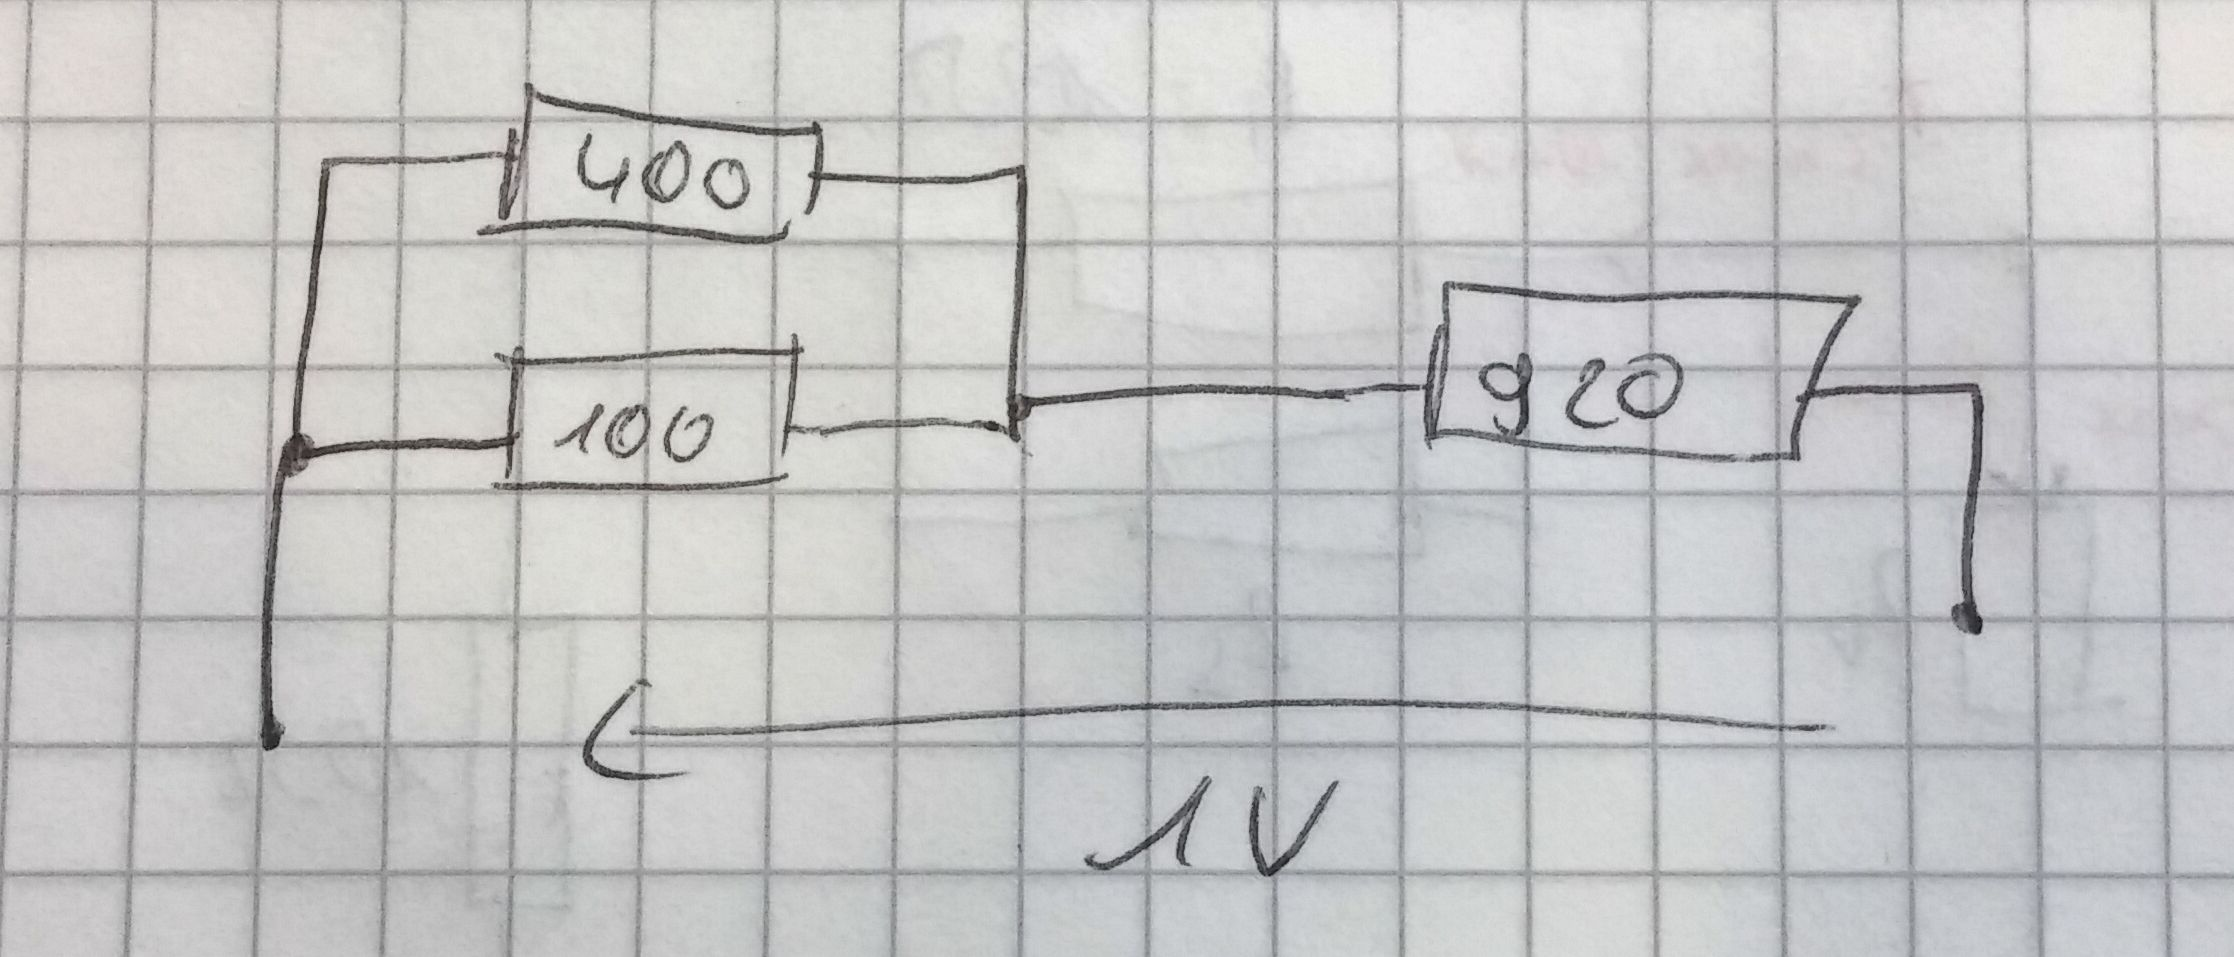
\includegraphics[scale=0.2]{A3_1_1.jpg}
\end{figure}



\begin{align*}
R_{ges} &= 920 + \frac{400 \cdot 100}{400 + 100} = \unit[1000]{\Omega}
\end{align*}


Von dem $\unit[920]{\Omega}$ fließen also \unit[1]{mA} nach links splittet sich dann wie im Aufgabenteil zuvor auf und wir erhalten dann wieder ein $I_{max} = \unit[0,2]{mA}$.

Bei einem $R_{ges} = \unit[100]{k \Omega}$ und $\unit[100]{V}$ haben wir genau die selbe Situation nur andere Werte.


\subsection*{d)}

Die Innenwiderstände sind wie folgt:

\begin{tabular}{|l|l|}
	\hline $\unit[100]{V}$ Messbereich & $\unit[100]{k\Omega}$  \\ 
	\hline $\unit[1]{V}$ Messbereich & $\unit[1]{k\Omega}$ \\ 
	\hline $\unit[1]{mA}$ Messbereich & $\unit[80]{\Omega}$ \\ 
	\hline $\unit[1]{A}$ Messbereich & $\unit[0,1]{\Omega}$ \\ 
	\hline 
\end{tabular} 

\section{Aufgabe 3.2}

Diese Aufgabe wurde nicht gemacht weil sie veraltet ist.

\newpage


\section{Aufgabe 3.3}

\begin{figure}[h]
	\centering
	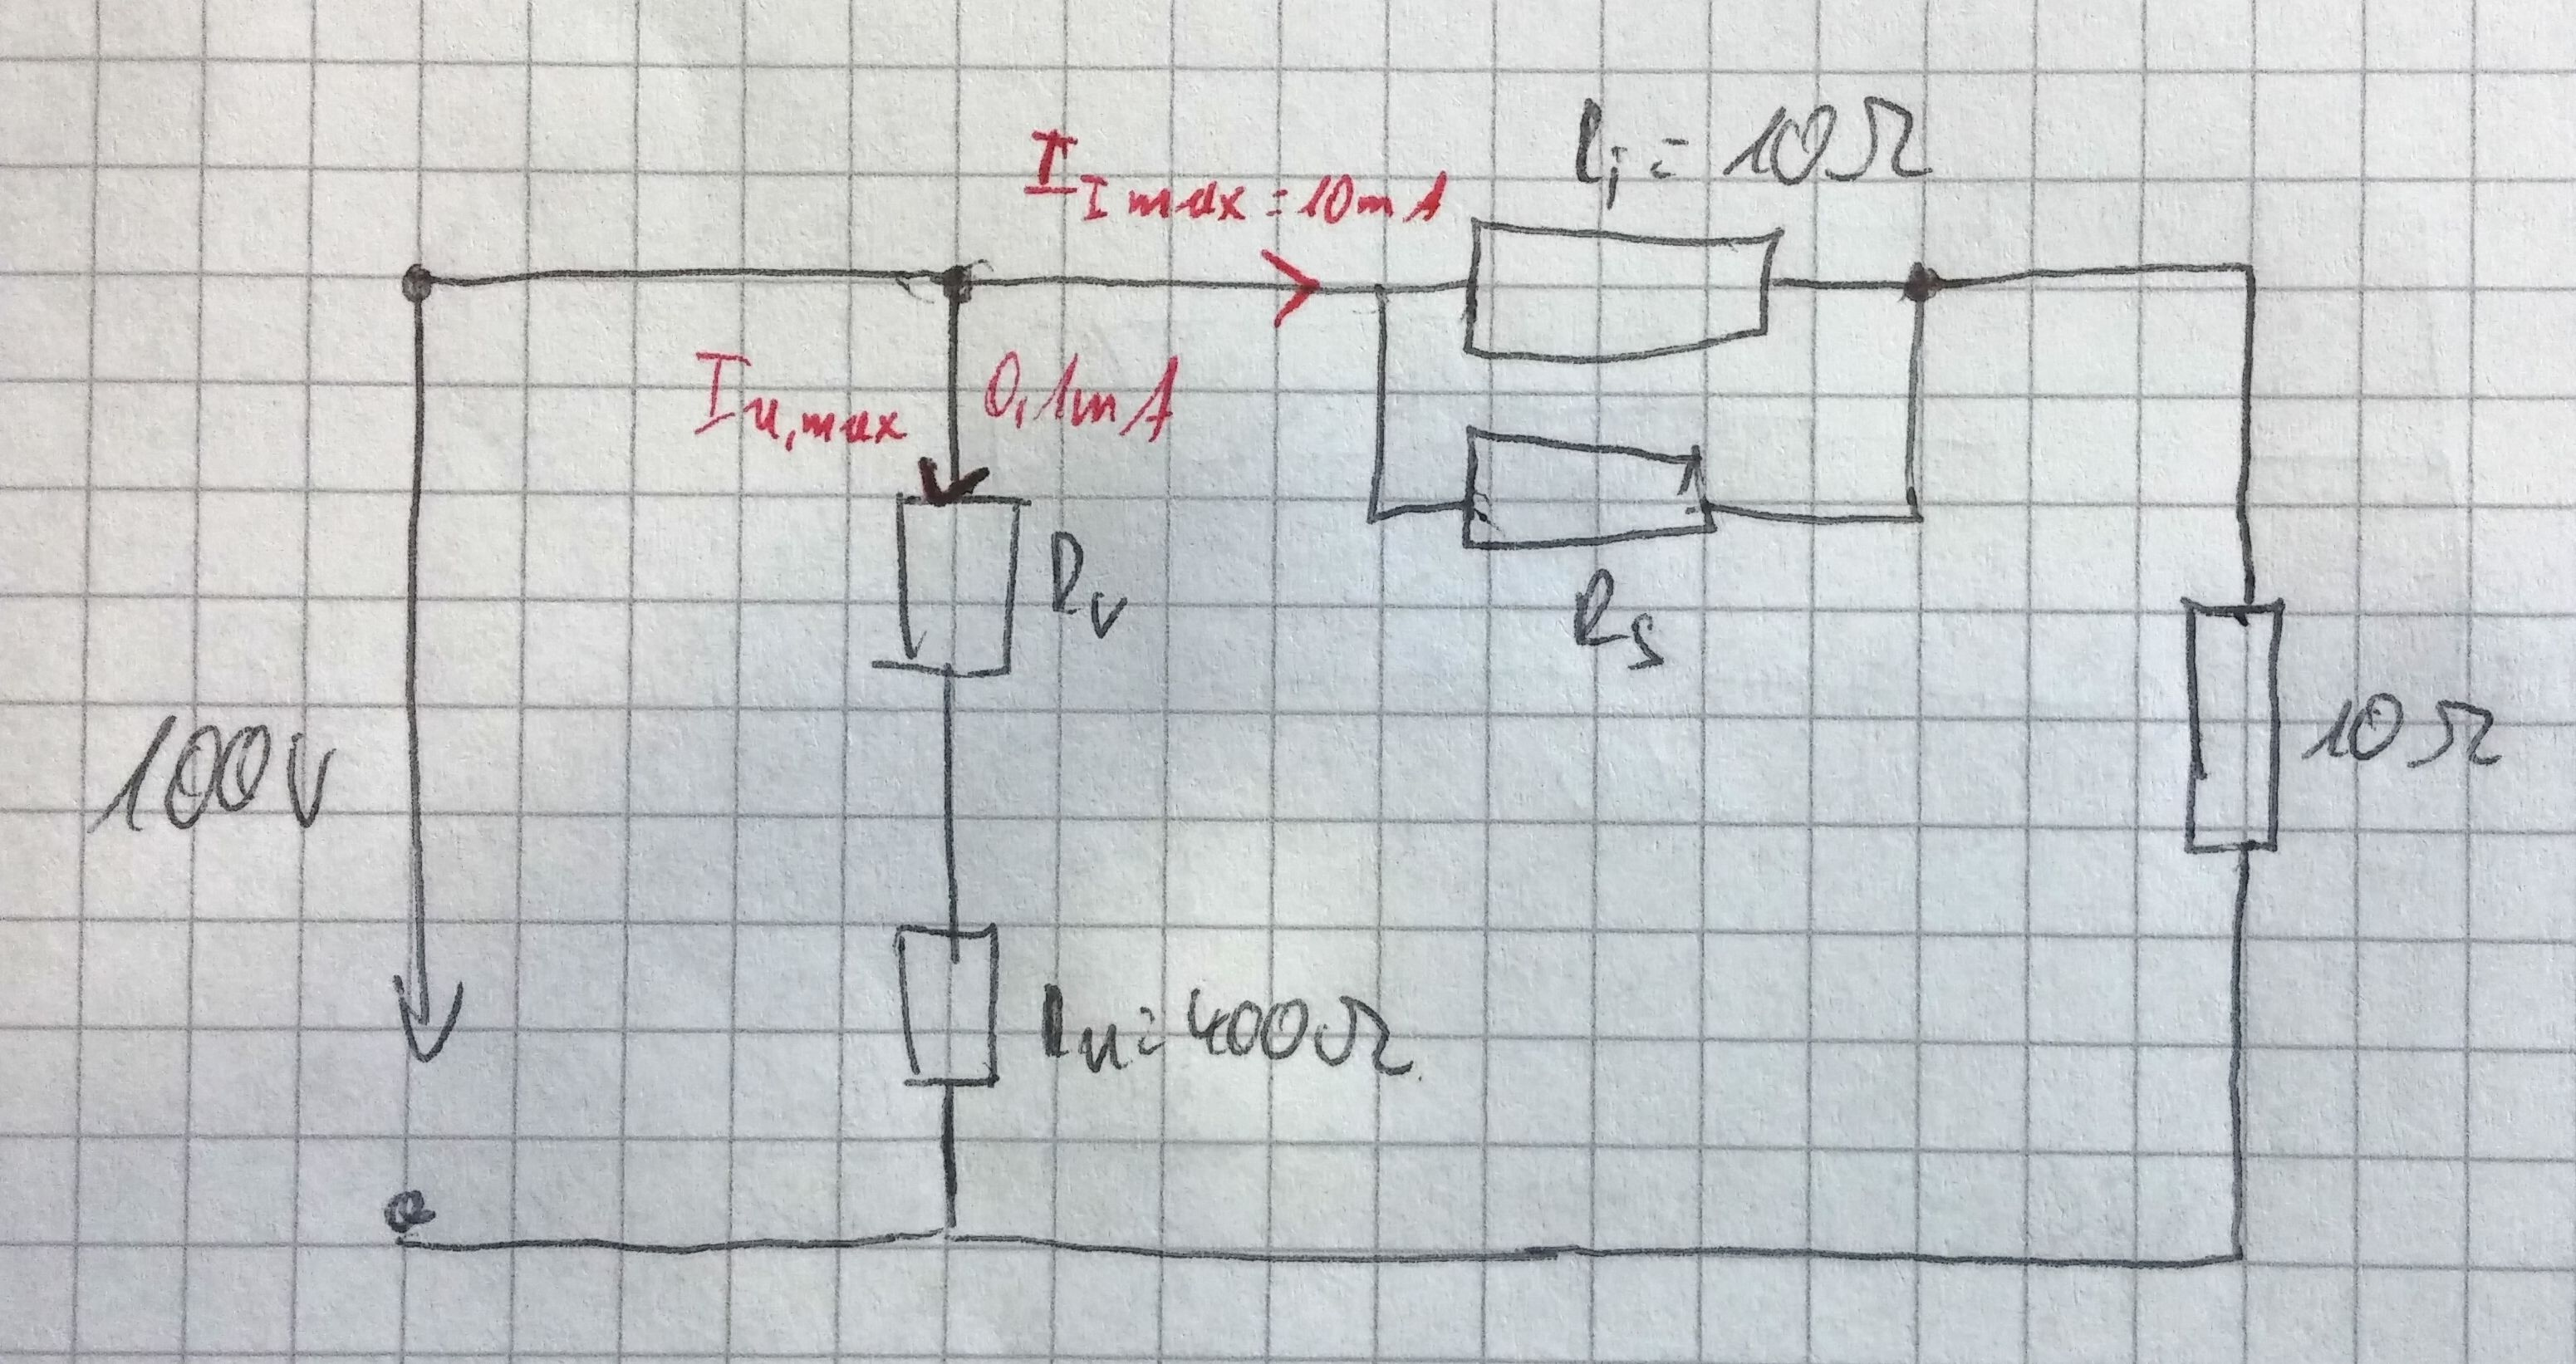
\includegraphics[scale=0.15]{A3_3_1.jpg}
\end{figure}




\begin{align*}
U &= \left( R_V + R_U \right) \cdot I_{U,max} \\
\Leftrightarrow R_V &= \frac{U - R_U \cdot I_{u,max}}{I_{u,max}} = \frac{U}{I_{u,max}} \cdot R_U = \frac{100}{0,1} \cdot 400 = \unit[1]{M \Omega}
\intertext{Nun bestimmen wir noch den Shuntwiderstand:}
\frac{I_S}{I_{I,max}} &= \frac{R_I}{R_S} \Leftrightarrow I_S = \frac{R_I}{R_S} \cdot I_{I,max} \\
I &= I_S + I_{I,max} = I_{I,max} \cdot \left( \frac{R_I}{R_S} + 1 \right) \\
R_S = R_I \cdot \frac{I_{I,max}}{I - I_{I,max}} &= \frac{\unit[10]{mA}}{\unit[10]{A} - \unit[10]{mA}} \cdot \unit[10]{\Omega} = \unit[0,01]{\Omega}
\end{align*}


















\end{document}